% Title page.
\title[Aula 01]{Ondas e Marés}
\author[Filipe Fernandes]{Filipe P. A. Fernandes}
\institute[unimonte]{Centro Universitário Monte Serrat}
\date[Agosto 2013]{09 de Agosto 2013}

\logo{
\includegraphics[scale=0.15]{../common/university_logo.png}}

\begin{document}

% The title page frame.
\begin{frame}[plain]
  \titlepage
  \begin{center}
    
\includegraphics[scale=0.5]{../common/by-nc-sa.pdf}
  \end{center}
\end{frame}

\section*{Outline}
\begin{frame}
\tableofcontents
\end{frame}


\section{Aula 01}
\subsection{Ementa}
\begin{frame}
    \frametitle{Ondas e Marés -- Carga horária: 60 h}
    {\small
    \begin{block}{Ementa}
        Introdução às oscilações da superfície do mar, Ondas superficiais de
        gravidade, ondas geradas pelo vento, teoria de ondas superficiais,
        dispersão e formação em grupo de ondas, ondas em aproximação da costa;
        principais processos costeiros (reflexão, difração, refração);
        Dispersão de energia e acoplamento ao transporte litorâneo (interação
        com a disciplina de Morfodinâmica Costeira); Marés: forças geradoras;
        interações entre marés lunares e solares; análise harmônica e marés reais.
    \end{block}
    }
\end{frame}

\begin{frame}
    \frametitle{Bibliografia}
    {\scriptsize
    {\bf Bibliografia Básica:}
        \begin{itemize}[<+-| alert@+>]
            \item GARRISON, Tom; MIYAJI, Cíntia (Trad.). Fundamentos de
                  oceanografia. São Paulo: Cengage Learning, 2009. 426 p.
                  ISBN 9788522106776
            \item NUSSENZVEIG. H. Moyses. Curso de física básica: volume 2:
                  fluidos, oscilações e ondas, calor. 4. ed. rev. São Paulo:
                  Edgar Blücher, 2002. xii, 328 p. ISBN 9788521202981
            \item SVERDRUP, K. A., Duxbury A. B., Duxbury, A. C. 2006.
                  Fundamentals of Oceanography. McGraw Hill, 5th edition.
                  Número de Chamada: 551.46 S968f 2006
        \end{itemize}
    }
\end{frame}

\begin{frame}
    \frametitle{Bibliografia}
    {\scriptsize
    {\bf Bibliografia Complementar:}
    \begin{itemize}[<+-| alert@+>]
        \item BOCAFOLI. Física: cinemática, estática e dinâmica. São Paulo:
              FTD, 1990. 238 p. ISBN 8532202926.
        \item HALLIDAY, David; RESNICK, Robert; WALKER, Jearl. Fundamentos de
              física: mecânica. 7. ed. Rio de Janeiro: LTC, 2006. v.1
        \item STEWART, R. H. 2002. Introduction to Physical Oceanography.
              Department of Oceanography. Texas A. M. University.
        \item The Open University. 1989. Ocean Circulation, Pergamon Press,
              2nd edition.
        \item WRIGHT, John R.; COLLING, Angela; PARK, Dave. Waves, tides, and
              shallow-water processes. 2. ed. Oxford: Boston: Butterworth
              Heinemann, in association with the Open University, 2006. 227 p.
    \end{itemize}
    }
\end{frame}

\begin{frame}
    \frametitle{Conversa}
    \begin{itemize}
        \item Lista com nomes e e-mails para contato;
        \item Interesses/Áreas/Estágios;
        \item Nível de Inglês;
        \item Nível de Computação;
        \item Nível de Matemática;
    \end{itemize}
\end{frame}

\begin{frame}
    \frametitle{Avaliações}
    \begin{itemize}
        \item 35 + 35 + {\bf 30}.
        \item {\bf 30} divididos entre 15 trabalhos e 15 {\bf Prova integradora};
        \item O aluno tem direito a uma prova alternativa (com o conteúdo de
              todo o semestre) para a menor nota.
    \end{itemize}
    \begin{block}{}
    Não há segunda chamada{\bf *} nem abono{\bf *}
    de falta não amparado por lei!
    \end{block}
\end{frame}

\section{Aula 01}
\subsection{Introdução}
{% Imagem de fundo local.
\usebackgroundtemplate{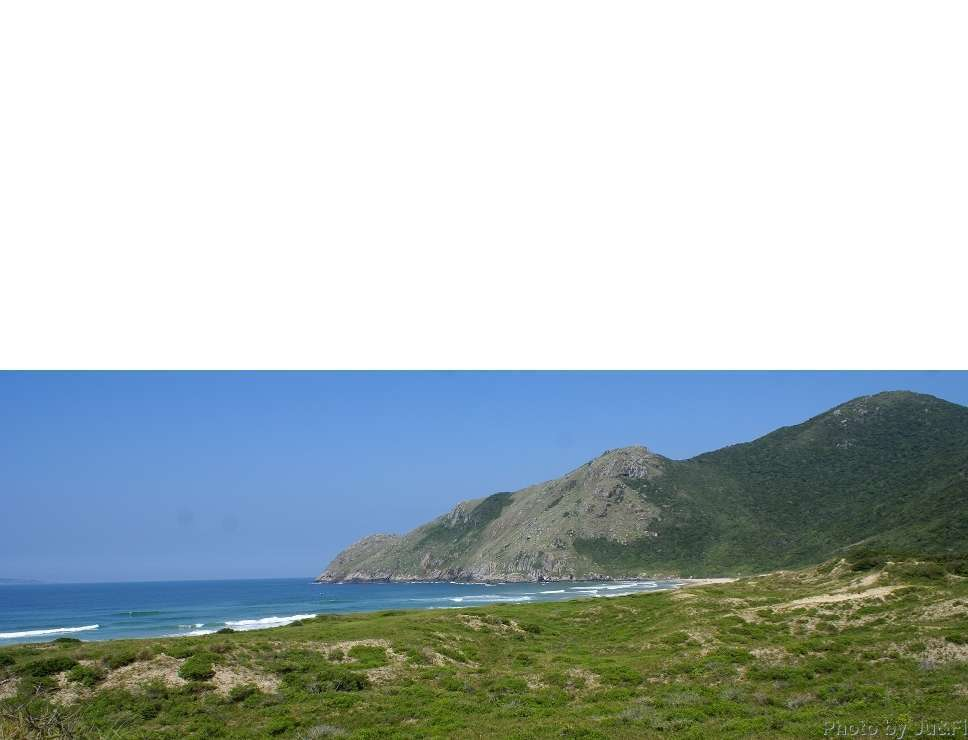
\includegraphics[width=\paperwidth]{./figures/santa_catarina.jpg}}
\begin{frame}
    \frametitle{Importância/Motivação}
    \begin{itemize}[<+-| alert@+>]
        \item Porque estudar as ondas no oceano?
        \item Algumas respostas:
            \begin{enumerate}[<+-| alert@+>]
                \item[] Engenharia costeira;
                \item[] Segurança de banhistas;
                \item[] Erosão costeira;
                \item[] Geração de energia.
            \end{enumerate}
        \item Eu enumerei apenas 4 itens, quem se habilita a expandir lista?
            % Navegação, Defesa/Segurança, Clima, Pesca, Recreação.
    \end{itemize}
    \vspace*{5cm}
\end{frame}
}

\subsection{Classificação de ondas}
\begin{frame}
    \frametitle{Classificação de ondas}
    \small{
    \begin{itemize}[<+-| alert@+>]
        \item Quanto à localização:
            \begin{enumerate}[<+-| alert@+>]
                \item[] Equatorial, Polar, Tropical
                \item[] {\bf Plataforma continental e Costerias}
                \item[] Canais
            \end{enumerate}
        \item Quanto à dinâmica:
            \begin{enumerate}[<+-| alert@+>]
                \item[] {\bf Curta/Longa}
                \item[] Interna/{\bf Externa}
            \end{enumerate}
        \item Quanto à força restauradora:
            \begin{enumerate}[<+-| alert@+>]
                \item[] Sonora
                \item[] Capilar
                \item[] {\bf Gravidade}
                \item[] Vorticidade
            \end{enumerate}
    \end{itemize}
        }
\end{frame}

\begin{frame}
    \frametitle{Classificação de ondas}
    \small{
    \begin{itemize}[<+-| alert@+>]
        \item Quanto à forçante:
            \begin{enumerate}[<+-| alert@+>]
                \item[] {\bf Atmosférica}
                \item[] Sísmica
                \item[] {\bf Gravitacional}
            \end{enumerate}
    \end{itemize}
    }
\end{frame}

\begin{frame}
    \frametitle{Espectro}
    \begin{center}
        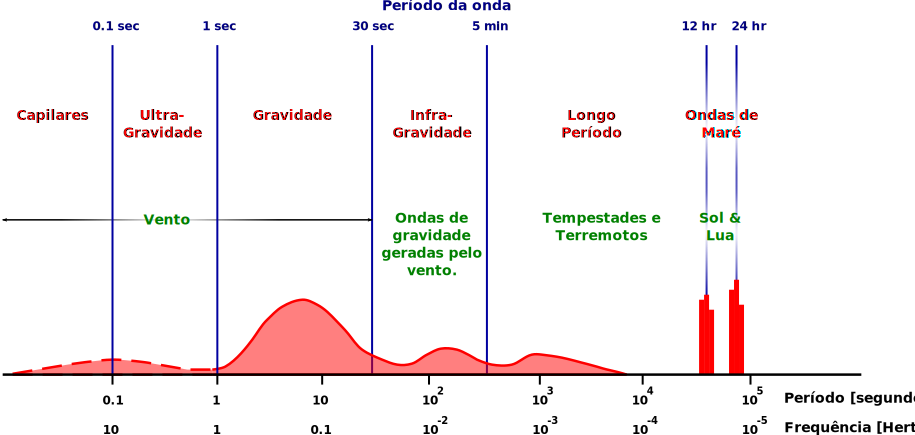
\includegraphics[scale=0.45]{./figures/Munk_ICCE_1950_Fig1.pdf}
%         http://en.wikipedia.org/wiki/File:Munk_ICCE_1950_Fig1.svg
%         FIXME: Original figure was `spectro.png` had waves when `f` is
%         important.  I belive was from Open University Book.
    \end{center}
\end{frame}

\begin{frame}
    \frametitle{Propriedade Fundamental}
    \begin{block}{}
        Ondas transportam {\bf energia} sem transportar uma quantidade
        {\bf significativa} de matéria.
    \end{block}
    \begin{center}
        \includegraphics[scale=0.3]{./figures/c10stokes2.jpg}
    \end{center}
\end{frame}

\subsection{Ondas como fonte de energia}
\begin{frame}
    \frametitle{Ondas como fonte de energia}
    \begin{columns}
        \begin{column}{0.5\textwidth}
        \small{
            \begin{itemize}[<+-| alert@+>]
                \item Ondas oceânicas representam uma fonte de energia limpa e
                      renovável;
                \item Essa energia é uma conversão do vento que sopra sobre os
                      oceanos...
                \item ... que por sua vez é uma conversão da energia solar.
                \item Fica a pergunta: {\it Porque não utilizar a energia do
                     vento ou solar diretamente?}
            \end{itemize}
            }
        \end{column}
        \begin{column}{0.5\textwidth}
            \begin{center}
                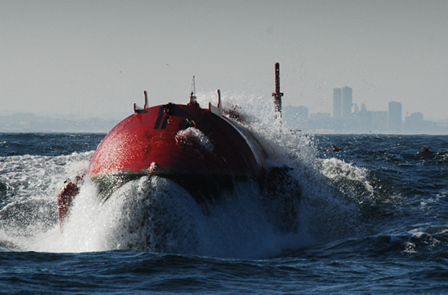
\includegraphics[scale=0.4]{./figures/Pelamis_bursts_out_of_a_wave.jpg}
%           http://en.wikipedia.org/wiki/File:Pelamis_bursts_out_of_a_wave.JPG
            \end{center}
        \end{column}
    \end{columns}
\end{frame}

\begin{frame}
    \frametitle{Ondas como fonte de energia}
        \footnotesize{
            \begin{itemize}[<+-| alert@+>]
                \item Maior disponibilidade, predicabilidade e baixo impacto
                      visual.
                \item A energia das ondas é 5$\times$ mais densa que a energia dos
                      ventos e 10-30 vezes mais que a energia solar;
                \item Alguns números:
                    \begin{enumerate}[<+-| alert@+>]
                        \item[] Energia solar: 100--200 W m$^{-2}$
                        \item[] Energia de vento: 400--600 W m$^{-2}$
                        \item[] Energia de ondas: 2--3 kW m$^{-2}$
                    \end{enumerate}
                \item $E = k_EH^2$, onde $k_E = \frac{\rho g}{8} \approx
                      1.25$ s m$^{-3}$
                \item Exemplo: $H = 2$ m $\rightarrow E = 5$ kW s m$^{-2}$
            \end{itemize}
            }
\end{frame}

\begin{frame}
    \frametitle{Ondas como fonte de energia}
    \begin{columns}
        \begin{column}{0.5\textwidth}
            \begin{center}
                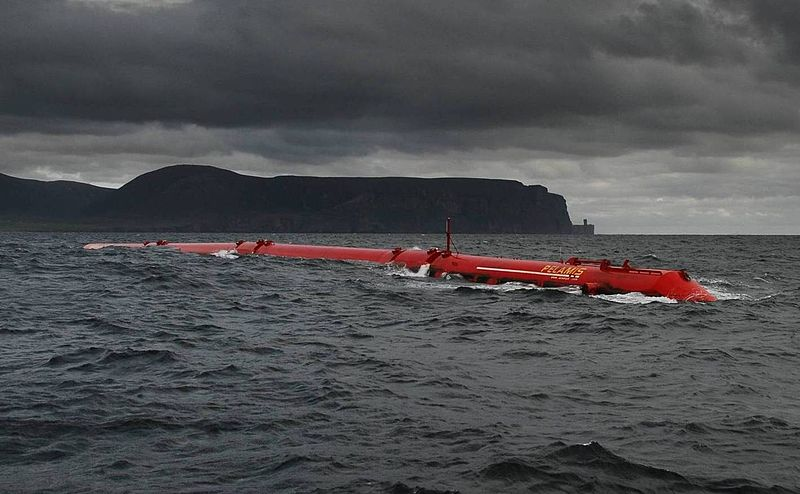
\includegraphics[width=\columnwidth]{./figures/800px-Pelamis_at_EMEC.jpg}
%                 http://en.wikipedia.org/wiki/File:Pelamis_at_EMEC.jpg
            \end{center}
        \end{column}
        \begin{column}{0.5\textwidth}
            \begin{center}
                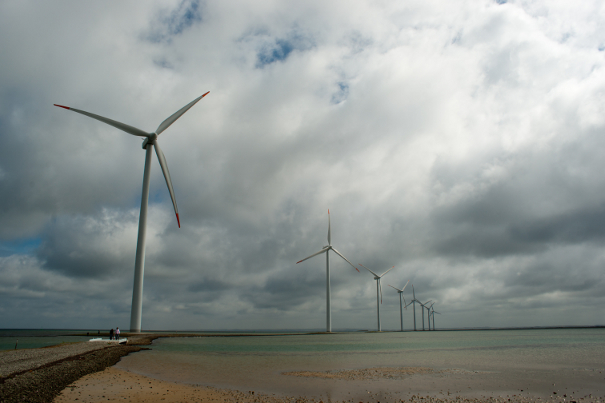
\includegraphics[width=\columnwidth]{./figures/ronland_windpark.jpg}
%                 http://en.wikipedia.org/wiki/File:R%C3%B8nland_Windpark.jpg
            \end{center}
        \end{column}
    \end{columns}
\end{frame}

\subsection{Impactos Ambientais}
\begin{frame}
    \frametitle{Impactos Ambientais}
    \small{
    \begin{itemize}[<+-| alert@+>]
        \item Cabos e sistemas de fundeio.
            \begin{enumerate}[<+-| alert@+>]
                \item[] A vida marinha pode ficar emaranhada?
            \end{enumerate}
        \item Campos eletromagnéticos.
            \begin{enumerate}[<+-| alert@+>]
                \item[] Já existem vários devido aos cabos de comunicação e
                        energia.
                \item[] A Vida marinha será atraída ou repelida?
            \end{enumerate}
        \item Ruído.
            \begin{enumerate}[<+-| alert@+>]
                \item[] Como se compara com o ruido de uma frota pesqueira?
            \end{enumerate}
    \end{itemize}
    }
\end{frame}

\begin{frame}
    \frametitle{Impactos Ambientais}
    \small{
    \begin{itemize}[<+-| alert@+>]
        \item Colisões.
            \begin{enumerate}[<+-| alert@+>]
                \item[] As locações e movimentos dos instrumentos óbvios para
                        a vida marinha?
            \end{enumerate}
        \item Efeito ``Coral Artificial''.
            \begin{enumerate}[<+-| alert@+>]
                \item[] Vida marinha vai se agregar ao redor dos instrumentos?
                \item[] Como isso afetaria o impacto local de um sistema
                        presa-predador?
            \end{enumerate}
    \end{itemize}
    }
\end{frame}

\begin{frame}
  \frametitle{Dever de casa -- Descrevendo uma onda}
    \begin{block}{}
        \url{http://pt.wikipedia.org/wiki/Onda}
        \[
          y=A(t,x)\cdot \cos (kx - \omega t + \phi)
        \]
    \end{block}
\end{frame}


{% Imagem de fundo local.
\usebackgroundtemplate{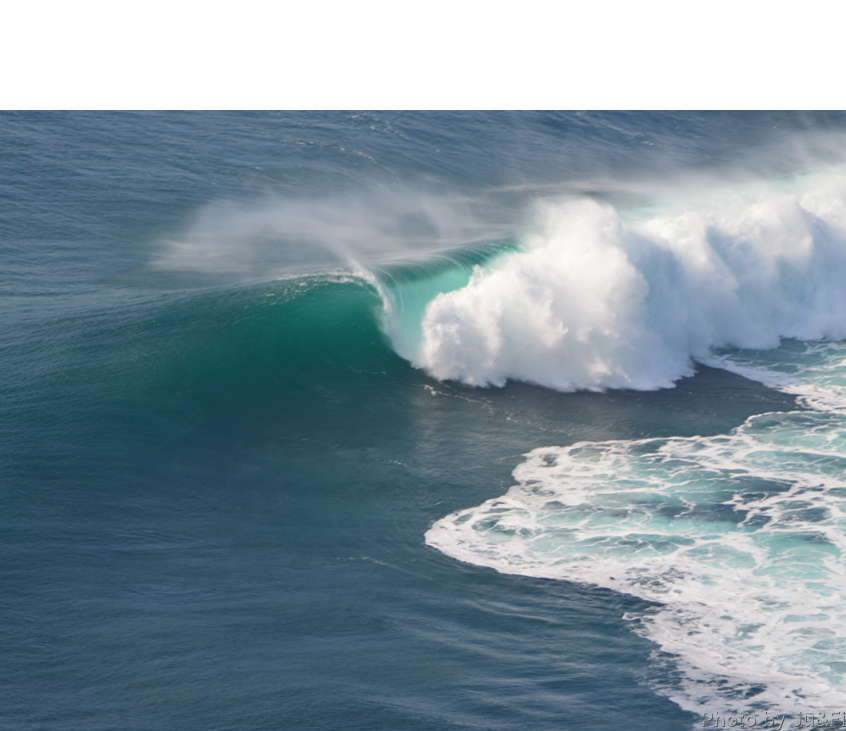
\includegraphics[width=\paperwidth]{./figures/ireland_wave.jpg}}
\begin{frame}
    \frametitle{Fim!}
        \begin{center}
            Perguntas?
        \end{center}
\vspace*{10cm}
\end{frame}
}

\end{document}
